\documentclass[11pt]{article}

\usepackage[a4paper,
bindingoffset=0.2in,
left=1in,
right=1in,
top=1in,
bottom=1in,
footskip=.25in]{geometry}
\usepackage{titlesec}
\usepackage{graphicx}
\usepackage{parskip}
\usepackage{tabularx}
\usepackage{float}
\usepackage{amsmath}
\newtheorem{assumption}{Assumption}
\usepackage{siunitx}
\usepackage[backend=biber,style=apa]{biblatex}
%\DeclareDelimFormat{nameyeardelim}{\addspace} 
\addbibresource{references.bib}

%opening
\title{Eosense Flux Chambers: Background and Theory}
\author{Emily Chua}

\begin{document}

\maketitle

\section{Original eosFD Theoretical Framework} \label{sec:orig}
\subsection{eosFD Overview}
The eosFD (Eosense Inc.) is a flux chamber system designed for high temporal-resolution monitoring of near-surface soil CO$_2$ fluxes. An eosFD Network consists of paired ``Soil" (hereafter called ``Sample") and ``Reference" Nodes that measure gas concentrations within enclosed chambers and use their difference to estimate a steady-state CO$_2$ flux (Table \ref{tab:terminology}). 

The eosFD operates using a forced diffusion approach \parencite{risk2011}, in which gas exchange between the chamber and its surroundings is regulated by hydrophobic membranes with known conductance. Each Node contains side-wall membranes that permit exchange with the atmosphere, while the Sample Node additionally includes a bottom membrane that allows exchange with the underlying surface. The Reference Node is capped at the base, preventing exchange and providing a real-time atmospheric correction. 

An equilibrium is established between gas entering the chamber through the bottom membrane and gas exiting through the side membranes. Measurements of gas concentration within each chamber are then used, together with known geometry and calibrated membrane properties, to estimate surface CO$_2$ flux.


\subsection{Concentration Measurement}
Gas-phase CO$_2$ concentrations within each eosFD chamber are measured using a non-dispersive infrared (NDIR) sensor housed within each Node (Fig. \ref{fig:flow-paths}). The sensor measures CO$_2$ gas concentration along with internal temperature and pressure, allowing concentrations to be expressed on a molar basis.

Gas diffuses through the chamber membranes and equilibrates within the chamber volume, where it is sampled continuously by the NDIR sensor. Like all optical gas sensors, NDIR sensors exhibit gradual drift over time due to changes in their electrical and mechanical properties. To account for this drift, Eosense recommends users periodically check calibration of the sensor using known concentration standards, including a zero-CO$_2$ gas (e.g., high-purity N$_2$) and a span gas ($\sim$1,000 ppm CO$_2$). 

Eosense calibrates concentration within the 0--30,000 ppm range, with an accuracy of $\pm$40 ppm within the 0--3,000 ppm range (Table \ref{tab:specs}). These measured gas-phase concentrations form the primary observables used in the flux calculations described below.


\subsection{Flux Estimation}
Flux across the membranes is driven by the concentration on either side and by the membrane's physical dimensions and diffusivity. The full differential equation is:

\begin{equation} \label{eq:1}
	\frac{V_m}{S} \frac{\partial C_s}{\partial t} = f_s(t) - D \frac{C_s - C_r}{L}
\end{equation}
where $V_m$ is the volume of the measuring chamber, $S$ is the surface area of the membrane, $\frac{\partial C_s}{\partial t}$ is the time rate of change of concentration in the chamber, $f_s(t)$ is the time-dependent flux rate from the sample, $C_s$ is the concentration in the Sample chamber, $C_r$ is the ambient concentration measured by the Reference chamber, $D$ is the diffusivity through the chamber volume and across the membrane to the atmosphere, and $L$ is the characteristic path length for gas diffusion through the membranes and chamber to the NDIR sensor (Fig. \ref{fig:flow-paths}).

Eosense flux estimates assume that the change in the head space concentration reaches steady state over the time span of the concentration measurements ($\sim$10 s):
\begin{equation*}
	\frac{\partial C_s}{\partial t} = 0
\end{equation*}
This steady-state assumption reduces the differential equation to a linear dependence. Because the diffusivity and path length are constant, they can be represented by a single coefficient, $G = D/L$, which can be empirically measured using a known flux source (see Sect. \ref{sub:eos-cal}).
\begin{equation} \label{eq:2}
	f_s = G(C_s - C_r)
\end{equation}
Flux is calibrated within 0--10 $\mu$mol m$^{-2}$ s$^{-1}$ range with a resolution of 0.2 $\mu$mol m$^{-2}$ s$^{-1}$ (Table \ref{tab:specs}).

\subsection{Eosense's Calibration Method} 
\label{sub:eos-cal}
Eosense calibrates for $G$ by using a flux generator where $F_s$ is known and rearranging Eq. \ref{eq:2}. While it is possible to measure $D$, it differs slightly between different batches of membranes. It is also possible to estimate $L$, but obstructions in the flowpath from the internal CO$_2$ sensor and complex geometries (side vs. bottom membranes) make it difficult. Therefore, Eosense deems it easiest to empirically measure the characteristic $G$ of each chamber. 

The average calibration coefficient provided by Eosense is $G = 0.0123$ $\mu$mol m$^{-2}$ s$^{-1}$ ppm$^{-1}$ (or since 1 ppm = 1 $\mu$mol mol$^{-1}$, units of mol m$^{-2}$ s$^{-1}$). From the ideal gas law for CO$_2$ at 25$^o$C:
\begin{equation*}
	V = \frac{RT}{P} = \frac{(\SI{8.314}{\kPa\L\per\mol\per\K})({\SI{298.15}{K}})}{\SI{101.325}{\kPa}} = \SI{0.02446}{\cubic\m\per\mol}
\end{equation*}

We can then convert $G$ to units of m s$^{-1}$:
\begin{equation*}
	\SI{0.0123}{\mol\per\square\m\per\s} \times \SI{0.02446}{\cubic\m\per\mol} = \boxed{ \SI{3.01e-4}{\m\per\s}}
\end{equation*}

Using an estimated path length of $L = 0.0318$ m (Table \ref{tab:eosense-values}), the membrane diffusivity is estimated as $D = G \cdot 
L = \SI{0.957e-5}{\square\m\per\s}$.

\begin{table}[H]
	\caption{Eosense terminology for an eosFD network, capable of high temporal resolution monitoring of surface CO$_2$ efflux.}
	\begin{tabularx}{\textwidth}{lX}
		\hline
		\textbf{Term} & \textbf{Description} \\
		\hline
		Sample Node & A node configured to measure gas emissions from the sampling surface (soil, water, or other substrate). Its bottom membrane is uncapped, allowing diffusive gas exchange with the measurement surface. \\
		
		Reference Node & A node configured to measure background (ambient) atmospheric gas concentrations. Its bottom membrane is capped, preventing gas exchange with the sampling surface. \\
		
		Pair or Network & A matched set consisting of one Sample Node and one Reference Node. Together, the differential concentration between the nodes can be used to calculate gas flux. \\
		
		Measuring chamber & A node's enclosed chamber in which gas concentration is measured. The membranes on the nodes provide a known and quantifiable gas conductance, restricting gas flow out of the chamber and enabling flux to be calculated from the rate of concentration change within the chamber over time.\\
		
		Collar & A 2.5 cm-long attachment fitted to the chamber that forms a gas-tight seal with the measurement surface. \\
		
		\hline
		\label{tab:terminology}
	\end{tabularx}
\end{table}

\begin{figure}[H]
	\centering
	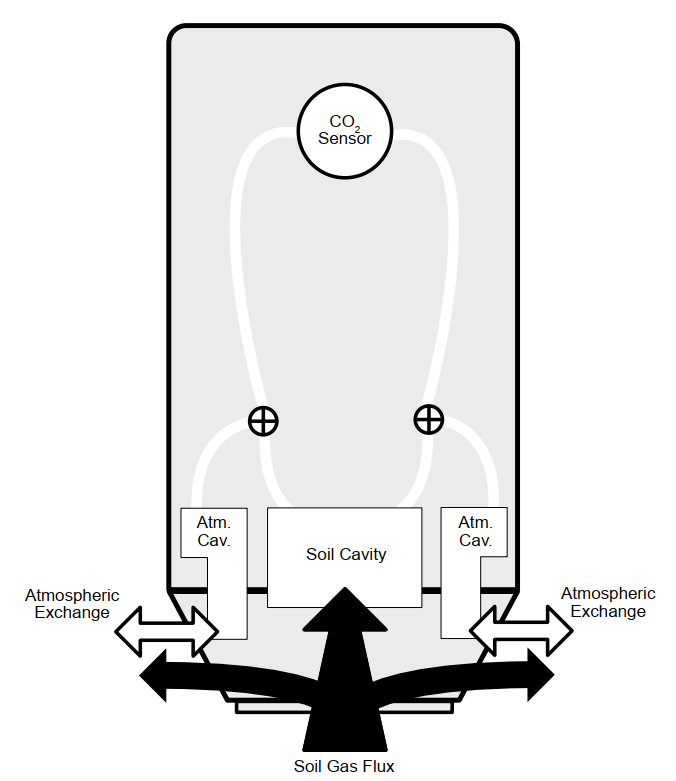
\includegraphics[width=.5\linewidth]{internal-cavity}
	\caption{Internal view of the eosFD chamber, depicting the exchange of atmospheric gases and soil (sample) flux with the chamber cavities. Source: \textcite{nickerson2018}.}
	\label{fig:flow-paths}
\end{figure}

\begin{table}[H]
	\caption{Performance specification details for the eosFDs, as provided by the Eosense manual.}
	\begin{tabularx}{\textwidth}{lX}
		\hline
		\textbf{Spec} & \textbf{Value} \\
		\hline
		Calibration range (concentration) & 0--30,000 ppm \\
		Calibration range (flux) & 0--10 $\mu$mol m$^{-2}$ s$^{-1}$ \\
		Concentration accuracy & 0--3,000 $\pm$ 40 ppm \newline 3,000--10,000 $\pm$ 2\% reading \newline Up to 30,000 $\pm$ 3.5\% reading \\
		Flux resolution & 0.2 $\mu$mol m$^{-2}$ s$^{-1}$ \\
		\hline
		\label{tab:specs}
	\end{tabularx}
\end{table}


\vspace{1cm}

\section{Reconsideration of eosFD Theory for Air--Sea Gas Flux Measurements} \label{sec:revised}
While Sect. \ref{sec:orig} summarizes the theoretical framework and equations as provided by Eosense, this section revisits these assumptions and reformulates the eosFD mass balance to reflect its operation when deployed over an air--water interface.

\begin{table}[H]
	\caption{Nomenclature of the relevant parameters for ultimately calculating the air--water CO$_2$ flux rate beneath the eosFD chamber.}
	\begin{tabularx}{\textwidth}{cXcc}
		\hline
		\textbf{Param.} & \textbf{Description} & \textbf{Units} & \textbf{Type} \\
		\hline
		
		$V_m$ & Volume of measuring chamber & m$^3$ & Known\\
		
		$V_c$ & Volume of collar & m$^3$ & Calculated\\
		
		$S_a$ & Total surface area of side membranes & m$^2$ & Known\\
		
		$S_c$ & Surface area of bottom membrane & m$^2$ & Known \\
		
		$S_w$ & Surface area of water covered by collar & m$^2$ & Known \\
		
		$C_a$ & Atmospheric CO$_2$ concentration & ppm & Measured \\
		
		$C_w$ & Waterside CO$_2$ concentration & ppm & Measured \\
		
		$C_s$ & CO$_2$ concentration in Sample Node chamber & ppm & Measured \\
		
		$C_r$ & CO$_2$ concentration in Reference Node chamber & ppm & Measured \\
		
		$C_c$ & CO$_2$ concentration in collar & ppm & Computed \\
			
		$k_a$ & Gas transfer velocity of side membrane & m s$^{-1}$ & Calibrated \\
		
		$k_c$ & Gas transfer velocity of bottom membrane & m s$^{-1}$ & Calibrated \\
		
%		$k_w$ & Gas transfer velocity of water within collar & m s$^{-1}$ & Computed \\
		
		$k_w^\dagger$ & ``True" gas transfer velocity of water (no chamber) & m s$^{-1}$ & Calibrated \\
		
		$f_a$ & CO$_2$ flux through Sample Node side membrane & mol m$^{-2}$ s$^{-1}$ & Intermediate \\
		
		$f_{a,r}$ & CO$_2$ flux through Reference Node side membrane & mol m$^{-2}$ s$^{-1}$ & Intermediate \\
		
		$f_c$ & CO$_2$ flux through bottom membrane & mol m$^{-2}$ s$^{-1}$ & Computed \\
		
		$f_w$ & CO$_2$ flux from water beneath chamber & mol m$^{-2}$ s$^{-1}$ & Computed \\
		
		$f_w^\dagger$ & ``True" CO$_2$ flux from water (no chamber) & mol m$^{-2}$ s$^{-1}$ & Computed \\
		
		\hline
		\label{tab:parameters}
	\end{tabularx}
\end{table}

\begin{table}[H]
	\caption{Eosense-provided values for relevant parameters in the flux calculations.}
	\begin{tabularx}{\textwidth}{cXXX}
		\hline
		\textbf{Param.} & \textbf{Description} & \textbf{Value} & \textbf{Source} \\
		\hline
		$G$ & Average membrane gas transfer velocity & 3.01 x 10$^{-4}$ m s$^{-1}$ & Calibration note \\
		$L$ & Estimated diffusion path length & 0.0318 m & Calibration note \\
		$S_a$ & Total surface area of side membranes & 804 mm$^2$ & Manual \\ 
		$S_c$ & Surface area of bottom membrane & 804 mm$^2$ & Manual \\
		$V_m$ & Volume of measuring chamber  & 16.7 cm$^3$ & Michelle Coleman's email (4/16/25) \\
		$V_c$ & Volume of collar & Diameter = 5 cm; length depends on water height & Dimensions from manual \\
		
		\hline
	\end{tabularx}
	\label{tab:eosense-values}
\end{table}

\begin{figure}[H]
	\includegraphics[width=1.0\linewidth]{Drawings/flux-chamber-diagram_V2}
	\caption{Diagram of an eosFD network (Sample and Reference Nodes), measuring over a water surface. Relevant parameters are shown, classified by whether they are known or must be calibrated, measured, or computed.}
	\label{fig:fluxchamber-diagram}
\end{figure}

\subsection{Non-Steady State Conditions}
Assuming that a continuous dynamic equilibrium exists between the water and atmosphere, the air--water CO$_2$ flux rate beneath the Sample chamber ($f_w$) can be derived by considering the mass balance within the 1) Sample Node measuring chamber, 2) Reference Node measuring chamber, and 3) Sample Node collar.

Note: In this section, all concentrations and fluxes ($C_a, C_s$, $f_a$, $f_c$, etc.) are functions of time (i.e., $C_a(t), C_s(t)$, $f_a(t)$, $f_c(t)$, etc.), but the explicit $t$-dependence is omitted for readability. Time dependence is made explicit again when solving the ODE for $C_c(t)$ (Eq. \ref{eq:16}).

\subsubsection{Mass balance within the measuring chambers}

The dynamic mass balance within the Sample Node's measuring chamber is as follows:
\begin{equation} \label{eq:3}
	V_m \frac{\partial C_s}{\partial t} = S_c f_c - S_a f_a
\end{equation}

Fick's Law gives the total CO$_2$ flux through the Sample Node side membranes:
\begin{equation} \label{eq:4}
	f_a = k_a(C_s - C_a)
\end{equation}

For the Reference Node, the bottom membrane membrane is sealed off, yielding the following dynamic mass balance:
\begin{equation} \label{eq:5}
	V_m \frac{\partial C_r}{\partial t} = -S_a f_{a,r}
\end{equation}

Fick's Law gives the total CO$_2$ flux through the Reference Node side membranes:
\begin{equation} \label{eq:6}
	f_{a,r} = k_a(C_r - C_a)
\end{equation}

Assuming $C_a$ is uniform, the flux through the bottom membrane can be derived as follows.

For the Sample Node, substitute Eq. \ref{eq:2} into Eq. \ref{eq:1}:
\begin{equation} \label{eq:7}
	V_m \frac{\partial C_s}{\partial t} = S_c f_c - S_a k_a (C_s - C_a)
\end{equation}

For the Reference Node, substitute Eq. \ref{eq:4} into Eq. \ref{eq:3}:
\begin{equation} \label{eq:8}
	V_m \frac{\partial C_r}{\partial t} = -S_a k_a (C_r - C_a)
\end{equation}

Combine the two time derivatives (Eq. \ref{eq:7} and \ref{eq:8}). This removes the dependence on $C_a$ and any bias from atmospheric variability, as the Reference Node acts as a real-time correction for atmospheric exchange.
\begin{equation} \label{eq:9}
	V_m \left(\frac{\partial C_s}{\partial t} - \frac{\partial C_r}{\partial t}\right) = S_c f_c - S_a k_a (C_s - C_r) 
\end{equation}

Finally, solve for $f_c$, noting that $S_a = S_c$:
\begin{equation} \label{eq:10}
	\boxed{f_c = \frac{V_m}{S_c} \left( \frac{\partial C_s}{\partial t} - \frac{\partial C_r}{\partial t} \right) + k_a (C_s - C_r)}
\end{equation}

This equation depends only on:
\begin{itemize}
	\item geometry ($S_c$, $V_m$),
	\item the eosFD-measured concentrations ($C_s$, $C_r$),
	\item their time derivatives ($\frac{\partial C_s}{\partial t}$, $\frac{\partial C_r}{\partial t}$), and
	\item the side-membrane gas transfer velocity ($k_a$), obtained via calibration (or using the averaged Eosense value; see Table \ref{tab:eosense-values}).
\end{itemize}

\subsubsection{Mass balance within the collar}

Similarly, the mass balance within the Sample Node collar is:
\begin{equation} \label{eq:11}
	V_c \frac{\partial C_c}{\partial t} = S_w f_w - S_c f_c
\end{equation}

The air--water CO$_2$ flux rate beneath the Sample chamber is given by the bulk flux equation,
\begin{equation} \label{eq:12}
	f_w = k_w(C_w - C_c)
\end{equation}

Fick's Law gives the CO$_2$ flux rate through the Sample Node bottom membrane:
\begin{equation} \label{eq:13}
	f_c = k_c(C_c - C_s)
\end{equation}

Substituting in Eqs. \ref{eq:12} and \ref{eq:13}, the equation governing the CO$_2$ concentration in the collar (Eq. \ref{eq:11}) can be rewritten as
\begin{equation} \label{eq:14}
	\frac{\partial C_c}{\partial t} + \left( \frac{S_w k_w}{V_c} + \frac{S_c k_c}{V_c} \right) C_c = \frac{S_w k_w}{V_c} C_w + \frac{S_c k_c}{V_c} C_s
\end{equation}

If we define the water-to-collar and  collar-to-chamber transfer rate constants as $\kappa_w = S_w k_w / V_c$ and $\kappa_c = S_c k_c / V_c$ (units: s$^{-1}$), respectively, Eq. \ref{eq:14}  becomes:

\begin{equation} \label{eq:15}
	\frac{\partial C_c}{\partial t} + ( \kappa_w + \kappa_c) C_c = \kappa_w C_w + \kappa_c C_s
\end{equation}

The general solution of the first-order, non-homogeneous linear differential equation (Eq. \ref{eq:15}) is given by the sum of the homogeneous and particular solutions:

\begin{equation} \label{eq:16}
	C_c(t) = Ae^{-(\kappa_w + \kappa_c)t} + \frac{\kappa_w C_w + \kappa_c C_s}{\kappa_w + \kappa_c}
\end{equation}

where $A$ is a constant defined by initial conditions. If the initial concentration in the collar at $t$ = 0 is $C_c(0) = C_a$, then $A$ is given by

\begin{equation} \label{eq:17}
	A = C_a - \frac{\kappa_w C_w^0 + \kappa_c C_s^0}{\kappa_w + \kappa_c}
\end{equation}

The final solution for the concentration in the collar is then
\begin{equation} \label{eq:18}
	\boxed{ C_c(t) = \left( C_a - \frac{\kappa_w C_w^0 + \kappa_c C_s^0}{\kappa_w + \kappa_c} \right) e^{-(\kappa_w + \kappa_c)t} + \frac{\kappa_w C_w + \kappa_c C_s}{\kappa_w + \kappa_c} }
\end{equation}

The time-dependent air--water CO$_2$ flux rate beneath the eosFD Sample chamber can then calculated using the bulk flux equation:
\begin{equation} \label{eq:19}
	\boxed{ f_w = k_w(C_w - C_c) }
\end{equation}

Eqs. \ref{eq:18} and \ref{eq:19} depend on:
\begin{itemize}
	\item known geometry ($S_w$, $S_c$, $V_c$),
	\item the eosFD Sample Node-measured CO$_2$ concentrations ($C_s^0$, $C_s$),
	\item the atmospheric CO$_2$ concentration ($C_a$), which must be measured with an external CO$_2$ sensor in air,
	\item the water CO$_2$ concentration ($C_w$), which must be measured with an external CO$_2$ sensor in water,
	\item the bottom-membrane gas transfer velocity ($k_c$), obtained via calibration, and
	\item the air--water gas transfer velocity beneath the chamber ($k_w$), which must be determined through analysis in the steady state (see next section).
\end{itemize}

\subsection{Steady-State Conditions}
In the steady state, we assume that
\begin{equation*}
	\dfrac{\partial C_s}{\partial t} = \dfrac{\partial C_r}{\partial t} = \dfrac{\partial C_c}{\partial t} = 0
\end{equation*}

From Eq. \ref{eq:8}, it follows that $C_r = C_a$.

This assumption yields a simplified expression for the CO$_2$ concentration in the collar, $C_c$:

\begin{equation}
	\left\{
	\begin{aligned}
		(\ref{eq:10}): f_c &= k_a\,(C_s - C_a) \\
		(\ref{eq:13}): f_c &= k_c\,(C_c - C_s)  \\
	\end{aligned}
	\right.
	\;\Longrightarrow\;
	C_c = C_s + \frac{k_a}{k_c}\,(C_s - C_r) \quad 
	\label{eq:20}
\end{equation}
which can then be used to calculate the gas transfer velocity beneath the collar:

\begin{equation}
	\left\{
	\begin{alignedat}{4}
		(\ref{eq:11}) \,&:\,&\quad S_w\,f_w \;=\;&\; S_c\,f_c \\
		(\ref{eq:13})\,&:\,&\quad f_c      \;=\;&\; k_c\,(C_c - C_s) \\
		(\ref{eq:19})\,&:\,&\quad f_w      \;=\;&\; k_w\,(C_w - C_c)
	\end{alignedat}
	\right.
	\;\Longrightarrow\;
	k_w \;=\; k_c\,\frac{S_c}{S_w}\,
	\frac{C_c - C_s}{C_w - C_c}
	\label{eq:21}
\end{equation}

We can now derive a simple expression for the steady-state true air--water CO$_2$ flux, $f_w^\dagger$.

To obtain an expression for the gas-transfer velocity, substitute Eq. \ref{eq:20} into Eq. \ref{eq:21}:
\begin{equation}\label{eq:22} 
	\boxed{k_w = \frac{\dfrac{S_c}{S_w}\,k_a} {\dfrac{C_w-C_s}{C_s-C_r}-\dfrac{k_a}{k_c}}}
\end{equation}

Assuming that $k_w^\dagger = k_w$, the bulk equation for the true air--water flux is:
\begin{equation}\label{eq:23}
	f_w^\dagger = k_w(C_w - C_a)
\end{equation}	
Substituting in Eq. \ref{eq:22}, we arrive at the steady-state true flux equation,
\begin{equation}\label{eq:24}
	\boxed{f_w^\dagger = \frac{\dfrac{S_c}{S_w}k_a(C_w - C_r)}{\dfrac{C_w - C_s}{C_s - C_r} - \dfrac{k_a}{k_c}}}
\end{equation}

Notes:
\begin{itemize}
	\item We can obtain $k_a, k_c$ from calibration of the side and bottom membranes.
	\item The eosFD Sample Node provides $C_s$.
	\item We must measure $C_w$ using an external water-side CO$_2$ sensor.
	\item The assumption that $C_r = C_a$ must be verified by comparing the eosFD Reference Node concentrations with that from an independent air-side CO$_2$ sensor.
	\item The derived expression for $k_w$ relies on the uniformity and accuracy of the measured $C_w$; water mixing must be sufficient to establish a homogeneous concentration field.
\end{itemize}


\subsection{Concentration-Based Calibration}
Our goal is to ultimately measure the air--water flux ($f_w$). To do so, we must calibrate the chambers to determine the transfer velocities through the side membranes ($k_a$) and bottom membrane ($k_c$).

To calibrate for the side membranes, we can use both the Sample and Reference Nodes. The Reference Node's dynamic mass balance is given by Eq. \ref{eq:5}. Similarly, if we cover the bottom membrane of the Sample Node, the mass balance within its measuring chamber follows from Eq. \ref{eq:3}:
\begin{subequations}\label{eq:25}
	\begin{align}
		\frac{V_m}{S_a} \frac{\partial C_r}{\partial t} = -k_a(C_r - C_a) \label{eq:a} \\
		\frac{V_m}{S_a} \frac{\partial C_s}{\partial t} = -k_a(C_s - C_a) \label{eq:b}		 
	\end{align}
\end{subequations}

To calibrate for the bottom membrane, we can cover the Sample Node's side membranes; given that in this setup $C_c = C_a$, Eq. \ref{eq:3} becomes
\begin{equation}\label{eq:26}
	\frac{V_m}{S_a} \frac{\partial C_s}{\partial t} = -k_c(C_s - C_a)
\end{equation}

For a constant $C_a$, the general solution to the first-order linear ODEs in Eq. \ref{eq:25} and \ref{eq:26} is
\begin{equation}\label{eq:27}
	C_m(t) = C_a + (C_m(0) - C_a)e^{-\gamma_i t}; \quad \gamma_i = \frac{S_i k_i}{V_m}
\end{equation}
where the subscript $m$ denotes either $s$ or $r$, depending on whether the Sample or Reference chamber is used for calibration, and the subscript $i$ denotes either $a$ or $c$ to refer to calibration of either the side (atmospheric) or bottom (collar) membranes. The exponent  $\gamma_i$ is a constant computed after fitting an exponential function to the sensor's time-response curve. Both $S_i$ and $V_m$ are provided by the manufacturer (Table \ref{tab:eosense-values}), enabling $k_i$ to be calculated.

In practice, electrical tape can be used to cover either the side or bottom membranes, and the eosFDs placed in a sealed environment in which the CO$_2$ concentration is increased from ambient conditions (e.g., 400--500 ppm) to a larger value (e.g., 900--1,000 ppm). Monitoring the exponential time response of the eosFDs to this step increase in CO$_2$ concentration over a sufficient time period enables an accurate fit to Eq. \ref{eq:27}. 

\subsubsection{Comparison to Eosense Calibration}
This calibration procedure differs in a key way from Eosense's. Their mass balance equation (Eq. \ref{eq:1}) implicitly assumes that the flux through the bottom membrane ($f_c$) is the same as the flux directly from the sample surface ($f_s$)---i.e., they ignore the collar flux---and they calibrate for $G$, which is the gas transfer velocity of the \textit{side membrane} (second term on the right in Eq. \ref{eq:1}). They also assume that $G$ is the same for the side and bottom membranes, which may not be true given that the path length from the side membrane to the NDIR sensor is not exactly the same as that from the bottom membrane to the sensor (Fig. \ref{fig:flow-paths}).

This can be illustrated as follows. From  Eqs. \ref{eq:3} and \ref{eq:5}, the Sample and Reference mass balances are, respectively:
\begin{equation*}
	V_m \frac{\partial C_s}{\partial t} = S_c f_c - S_a f_a
\end{equation*}
\begin{equation*}
	\frac{\partial C_r}{\partial t} = -S_a f_{a,r}
\end{equation*}

Eosense assumes steady-state conditions: $\dfrac{\partial C_s}{\partial t} = \dfrac{\partial C_r}{\partial t} = 0$.

The Sample mass balance becomes
\begin{equation*}
	f_c = f_a
\end{equation*}
and similarly for the Reference mass balance:
\begin{gather*}
	S_a k_a(C_r - C_a) = 0 \\
	\implies C_r = C_a
\end{gather*}

Here, Eosense assumes that $f_c = f_s$, and prescribes this flux during their calibration. Given these assumptions, the Sample mass balance becomes:
\begin{equation*}
	f_s = f_c = f_a = k_a(C_s - C_a)
\end{equation*}
But in steady state, $C_a = C_r$; therefore,
\begin{equation*}
	f_s = k_a(C_s - C_r)
\end{equation*}
which is identical to Eq. \ref{eq:2}, hence $G = k_a$; i.e., their calibration coefficient is equivalent to the side-membrane gas transfer velocity.

\subsection{Uncertainty Analysis}
The total measurement error contains systematic (aka ``bias") errors and random (aka ``precision") errors \parencite{figliola2019}. The systematic errors bias the sample mean from the true value by a fixed amount, while the random errors cause a distribution of measured values around the sample mean. 

Each individual measurement error interacts with other errors to affect the overall uncertainty---this is known as uncertainty propagation. Individual errors can be combined via the root-sum-squares (RSS) method:
\begin{equation} \label{eq:28}
	\begin{aligned}
	u_x &= \sqrt{u_1^2 + u_2^2 + ... + u_k^2} \\
		&= \sqrt{\sum_{k=1}^K u_k^2}
\end{aligned}
\end{equation}
where $u_k$ is the uncertainty of elements $k = 1, 2,..., K$.

\subsubsection{Systematic Error}
We account for the systematic error by determining the mean offsets between the eosFD Reference and Sample and Pro-Oceanus air-side CO$_2$ concentration measurements during offset tests ($\overline{C_r - C_a}$ and $\overline{C_s - C_a}$, respectively), and correcting subsequent data sets with these values before proceeding with the $k_w$ and flux analysis.

\subsubsection{Random Error}
For the random error, which arises from multiple variables---the calibration coefficients ($k_a, k_c$) and the measured concentrations ($C_w, C_s, C_r$)---we can determine the overall contribution of individual errors by propagating uncertainty through Eq. \ref{eq:22}:
\begin{equation} \label{eq:29}
	\sigma_{k_w}^2 = 
	\left(\frac{\partial k_w}{\partial k_a}\sigma_{k_a}\right)^2 + \left(\frac{\partial k_w}{\partial k_c}\sigma_{k_c}\right)^2 +
	\left(\frac{\partial k_w}{\partial C_w}\sigma_{C_w}\right)^2 +
	\left(\frac{\partial k_w}{\partial C_r}\sigma_{C_r}\right)^2 +
	\left(\frac{\partial k_w}{\partial C_s}\sigma_{C_s}\right)^2
\end{equation}

Determining $\sigma_{f_w^\dagger}$ requires differentiating Eq. \ref{eq:22} with respect to each parameter. First, simplify notation and define
\begin{equation}
	\left\{
	\begin{aligned}
		A &= S_c/S_w\\
		D &= \frac{C_w - C_s}{C_s - C_r} - \frac{k_a}{k_c}\\
		  &= B - \frac{k_a}{k_c}\\
			\end{aligned}
		\right.
		\;\Longrightarrow\;
		k_w = A \frac{k_a}{D} \quad 
\end{equation}

Using these simplifications, we take derivatives with respect to $k_a$ and $k_c$:

i) 
\begin{equation*}
	\begin{aligned}
	\frac{\partial k_w}{\partial k_a}
	&= \frac{AD + A\frac{k_a}{k_c}}{D^2}\\ 
	&= \frac{A(B-\frac{k_a}{k_c}) + A\frac{k_a}{k_c}}{D^2} = \frac{A B}{D^2}\\
	&= \frac{A \frac{C_w - C_s}{C_s - C_r}}{D^2}
	\end{aligned}
\end{equation*}

ii)
\begin{equation*}
	\begin{aligned}
	\frac{\partial k_w}{\partial k_c} 
	&= \frac{-\frac{k_a}{k_c^2} A k_a}{D^2}\\
	&= -A \frac{k_a^2}{k_c^2 D^2}
	\end{aligned}
\end{equation*}

For the concentration derivatives (with respect to $C_w, C_s$, and $C_r$):

iii)
\begin{equation*}
	\begin{aligned}
	\frac{\partial k_w}{\partial C_w} 
	&= \frac{-\frac{\partial D}{\partial C_w}Ak_a}{D^2}\\
	&= -\frac{Ak_a}{(C_s - C_r)D^2}
	\end{aligned}
\end{equation*}

iv)
\begin{equation*}
	\begin{aligned}
		\frac{\partial k_w}{\partial C_s} 
		&= \frac{-\frac{\partial D}{\partial C_s}Ak_a}{D^2}\\
		&= \frac{Ak_a(C_w-C_r)}{(C_s-C_r)^2 D^2}
	\end{aligned}
\end{equation*}

v) 
\begin{equation*}
	\frac{\partial k_w}{\partial C_r} 
		= \frac{-Ak_a(C_w-C_s)}{(C_s-C_r)^2D^2}
\end{equation*}

Then, $\sigma_{k_w} = \sqrt{(i)^2 + (ii)^2 + (iii)^2 + (iv)^2 + (v)^2}$.

Having calculated the uncertainty in $k_w$, we can now estimate the uncertainty in the true flux, $f_w^\dagger$ by similarly propagating uncertainty through Eq. \ref{eq:24}:
\begin{equation*}
		\sigma_{f_w^\dagger}^2 
		= \left(\frac{\partial f_w^\dagger}{\partial_w}\sigma_{k_w}\right)^2
		+ \left(\frac{\partial f_w^\dagger}{\partial C_w}\sigma_{C_w}\right)^2
		+ \left(\frac{\partial f_w^\dagger}{\partial C_a}\sigma_{C_a}\right)^2
\end{equation*}
\begin{equation*}
	\rightarrow \sigma_{f_w^\dagger} = \sqrt{((C_w-C_a)\sigma_{k_w})^2 + (k_w\sigma_{C_w})^2 + (k_w\sigma_{C_a})^2} m 
\end{equation*}

\subsection{Flux comparison}
In the flux analysis, we calculate four different fluxes: the flux through the bottom membrane $f_c$ (Eq. \ref{eq:10}), the air--water flux beneath the chamber $f_w$ (Eq. \ref{eq:19}), the ``true" air--water flux $f_w^\dagger$ (Eq.\ref{eq:24}), and an independent estimate of the true air--water flux from the water inventory $f_{w,PO} = -h \frac{dC_w}{dt}$. The fluxes that should agree are:

1. $f_w^{\dagger}$ and $f_{w,PO}$ \\
Both are intended to estimate the true air--water flux. Therefore, during pseudo-steady state, we should see
\begin{equation*}
	f_w^{\dagger} \approx f_{w,PO}
\end{equation*}

2. $f_c$ and $f_w$ \\
These are connected by the collar mass balance (Eq. \ref{eq:11}).
In steady state, $S_w f_w \approx S_c f_c \rightarrow f_w \approx \frac{S_c}{S_w} f_c$. Therefore,
\begin{equation*}
	f_w \approx 0.4095 f_c
\end{equation*}

\printbibliography

\end{document}
